% Options for packages loaded elsewhere
\PassOptionsToPackage{unicode}{hyperref}
\PassOptionsToPackage{hyphens}{url}
\PassOptionsToPackage{dvipsnames,svgnames*,x11names*}{xcolor}
%
\documentclass[
  10pt,
]{article}
\usepackage{amsmath,amssymb}
\usepackage{lmodern}
\usepackage{setspace}
\usepackage{iftex}
\ifPDFTeX
  \usepackage[T1]{fontenc}
  \usepackage[utf8]{inputenc}
  \usepackage{textcomp} % provide euro and other symbols
\else % if luatex or xetex
  \usepackage{unicode-math}
  \defaultfontfeatures{Scale=MatchLowercase}
  \defaultfontfeatures[\rmfamily]{Ligatures=TeX,Scale=1}
  \setmainfont[]{Georgia}
\fi
% Use upquote if available, for straight quotes in verbatim environments
\IfFileExists{upquote.sty}{\usepackage{upquote}}{}
\IfFileExists{microtype.sty}{% use microtype if available
  \usepackage[]{microtype}
  \UseMicrotypeSet[protrusion]{basicmath} % disable protrusion for tt fonts
}{}
\makeatletter
\@ifundefined{KOMAClassName}{% if non-KOMA class
  \IfFileExists{parskip.sty}{%
    \usepackage{parskip}
  }{% else
    \setlength{\parindent}{0pt}
    \setlength{\parskip}{6pt plus 2pt minus 1pt}}
}{% if KOMA class
  \KOMAoptions{parskip=half}}
\makeatother
\usepackage{xcolor}
\IfFileExists{xurl.sty}{\usepackage{xurl}}{} % add URL line breaks if available
\IfFileExists{bookmark.sty}{\usepackage{bookmark}}{\usepackage{hyperref}}
\hypersetup{
  pdftitle={ANTsX neuroimaging-derived structural phenotypes of UK Biobank},
  pdfauthor={N. Tustison, et al.},
  colorlinks=true,
  linkcolor={Maroon},
  filecolor={Maroon},
  citecolor={Blue},
  urlcolor={blue},
  pdfcreator={LaTeX via pandoc}}
\urlstyle{same} % disable monospaced font for URLs
\usepackage[margin=1.0in]{geometry}
\usepackage{graphicx}
\makeatletter
\def\maxwidth{\ifdim\Gin@nat@width>\linewidth\linewidth\else\Gin@nat@width\fi}
\def\maxheight{\ifdim\Gin@nat@height>\textheight\textheight\else\Gin@nat@height\fi}
\makeatother
% Scale images if necessary, so that they will not overflow the page
% margins by default, and it is still possible to overwrite the defaults
% using explicit options in \includegraphics[width, height, ...]{}
\setkeys{Gin}{width=\maxwidth,height=\maxheight,keepaspectratio}
% Set default figure placement to htbp
\makeatletter
\def\fps@figure{htbp}
\makeatother
\setlength{\emergencystretch}{3em} % prevent overfull lines
\providecommand{\tightlist}{%
  \setlength{\itemsep}{0pt}\setlength{\parskip}{0pt}}
\setcounter{secnumdepth}{5}
\usepackage{longtable}
\usepackage{graphicx}
\usepackage{booktabs}
\usepackage{textcomp}
\usepackage{xcolor}
\usepackage{geometry}
\usepackage{subcaption}
\definecolor{listcomment}{rgb}{0.0,0.5,0.0}
\definecolor{listkeyword}{rgb}{0.0,0.0,0.5}
\definecolor{listnumbers}{gray}{0.65}
\definecolor{listlightgray}{gray}{0.955}
\definecolor{listwhite}{gray}{1.0}
\setlength\tabcolsep{1.5pt}
\ifLuaTeX
  \usepackage{selnolig}  % disable illegal ligatures
\fi

\title{ANTsX neuroimaging-derived structural phenotypes of UK Biobank}
\author{N. Tustison, et al.}
\date{}

\begin{document}
\maketitle

{
\hypersetup{linkcolor=}
\setcounter{tocdepth}{2}
\tableofcontents
}
\setstretch{1.}
\clearpage

\hypertarget{age}{%
\section{Age}\label{age}}

\begin{figure}
\centering
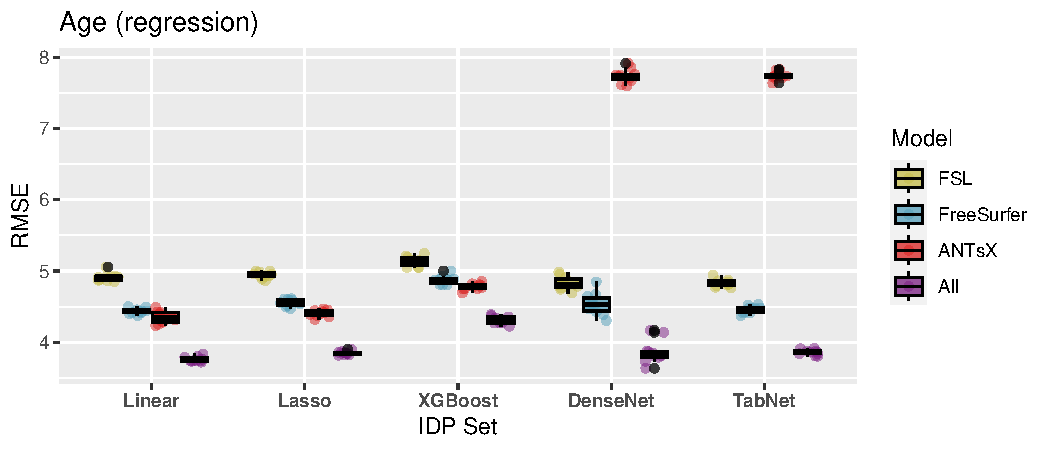
\includegraphics{/Users/ntustison/Documents/Academic/InProgress/ANTsXUKBB/Text/Figures/compare_predictions_Age.pdf}
\caption{Age}
\end{figure}

\hypertarget{feature-ranking-linear}{%
\subsection{Feature ranking: Linear}\label{feature-ranking-linear}}

\begin{table}

\caption{\label{tab:compare-predictions}Age}
\centering
\begin{tabular}[t]{lll}
\toprule
Package & Pipeline & Feature\\
\midrule
ANTsX & Atropos & Cerebellum\\
FreeSurfer & ASEG & Volume of WM-hypointensities (whole brain)\\
ANTsX & Cereb & L\_III volume\\
FreeSurfer & ASEG & Volume of CerebralWhiteMatter (left hemisphere)\\
FreeSurfer & ASEG & Volume of CerebralWhiteMatter (right hemisphere)\\
\addlinespace
FreeSurfer & ASEG & Volume of CC-Central (whole brain)\\
FreeSurfer & ASEG & Volume of SupraTentorial (whole brain)\\
FSL & Other & Continuous    Volume of grey matter\\
FreeSurfer & ASEG & Volume of TotalGray (whole brain)\\
FreeSurfer & ASEG & Volume of Cortex (left hemisphere)\\
\addlinespace
FreeSurfer & ASEG & Volume of VentricleChoroid (whole brain)\\
FreeSurfer & ASEG & Volume of Cortex (right hemisphere)\\
ANTsX & Cereb & CerebellarCSF volume\\
FreeSurfer & ASEG & Volume of VentralDC (right hemisphere)\\
ANTsX & Region & Right cerebellum exterior\\
\addlinespace
FreeSurfer & ASEG & Volume of VentralDC (left hemisphere)\\
ANTsX & Cereb & CerebellarWhiteMatter volume\\
FreeSurfer & ASEG & Volume of SubCortGray (whole brain)\\
ANTsX & Region & Cerebellar vermal lobules VI VII\\
ANTsX & Region & Left caudate\\
\addlinespace
FreeSurfer & ASEG & Volume of Amygdala (right hemisphere)\\
ANTsX & Region & Right lateral ventricle\\
ANTsX & Atropos & BrainStem\\
FreeSurfer & ASEG & Volume of Cerebellum-Cortex (left hemisphere)\\
FreeSurfer & ASEG & Volume of Caudate (left hemisphere)\\
\bottomrule
\end{tabular}
\end{table}

\begin{itemize}
\item
  FSL

  \begin{itemize}
  \item
    range: {[} NA , NA {]}
  \item
    std: NA
  \item
    skewness: NA
  \end{itemize}
\item
  FreeSurfer

  \begin{itemize}
  \item
    range: {[} 0.1526888 , 15.03373 {]}
  \item
    std: 2.686921
  \item
    skewness: 2.324572
  \end{itemize}
\item
  ANTsX

  \begin{itemize}
  \item
    range: {[} 0.1354494 , 17.57277 {]}
  \item
    std: 2.308719
  \item
    skewness: 2.238218
  \end{itemize}
\end{itemize}

\hypertarget{package-based-ranking-top-10-features}{%
\subsubsection{Package-based ranking (top 10
features)}\label{package-based-ranking-top-10-features}}

\begin{itemize}
\item
  FSL: rank = 363 , imp = 77.09145
\item
  FreeSurfer: rank = 80 , imp = 121.5785
\item
  ANTsX: rank = 166 , imp = 108.6568
\end{itemize}

\hypertarget{package-based-ranking-top-25-features}{%
\subsubsection{Package-based ranking (top 25
features)}\label{package-based-ranking-top-25-features}}

\begin{itemize}
\item
  FSL: rank = 1615 , imp = 155.1536
\item
  FreeSurfer: rank = 561 , imp = 241.8775
\item
  ANTsX: rank = 919 , imp = 205.7617
\end{itemize}

\hypertarget{package-based-ranking-top-50-features}{%
\subsubsection{Package-based ranking (top 50
features)}\label{package-based-ranking-top-50-features}}

\begin{itemize}
\item
  FSL: rank = 5368 , imp = 248.9677
\item
  FreeSurfer: rank = 3346 , imp = 355.6919
\item
  ANTsX: rank = 3177 , imp = 331.0176
\end{itemize}

\clearpage

\hypertarget{fluidintelligencescore}{%
\section{FluidIntelligenceScore}\label{fluidintelligencescore}}

\begin{figure}
\centering
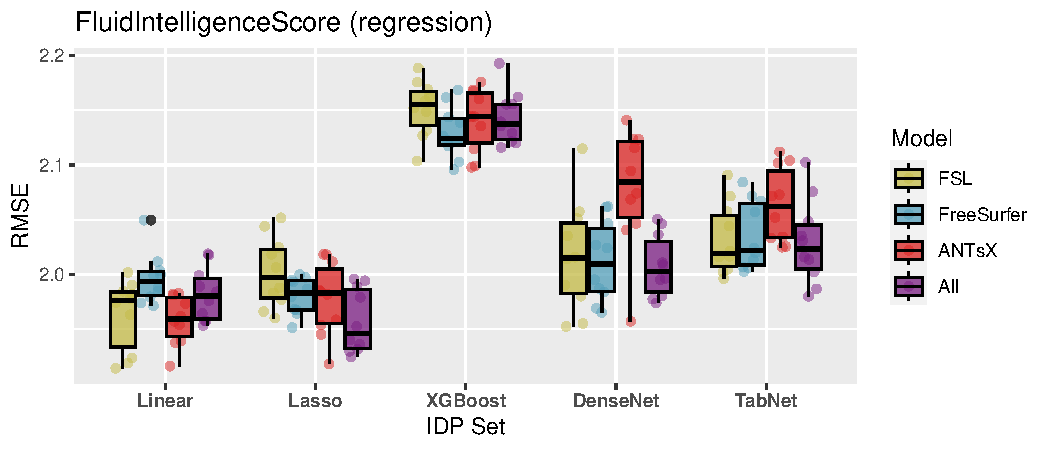
\includegraphics{/Users/ntustison/Documents/Academic/InProgress/ANTsXUKBB/Text/Figures/compare_predictions_FluidIntelligenceScore.pdf}
\caption{FluidIntelligenceScore}
\end{figure}

\hypertarget{feature-ranking-linear-1}{%
\subsection{Feature ranking: Linear}\label{feature-ranking-linear-1}}

\begin{table}

\caption{\label{tab:compare-predictions}FluidIntelligenceScore}
\centering
\begin{tabular}[t]{lll}
\toprule
Package & Pipeline & Feature\\
\midrule
FSL & FAST & Volume of grey matter in Amygdala (right)\\
FreeSurfer & ASEG & Volume of CC-Mid-Anterior (whole brain)\\
ANTsX & Thickness & Left paracentral\\
FSL & FAST & Volume of grey matter in Intracalcarine Cortex (right)\\
FSL & Other & Continuous    Volume of peripheral cortical grey matter\\
\addlinespace
ANTsX & Thickness & Left superior frontal\\
FSL & FAST & Volume of grey matter in Amygdala (left)\\
ANTsX & Thickness & Left inferior temporal\\
FSL & FAST & Volume of grey matter in Middle Temporal Gyrus - posterior division (left)\\
ANTsX & Region & Left hippocampus\\
\addlinespace
FreeSurfer & Thickness & Mean thickness of superiorparietal (left hemisphere)\\
FreeSurfer & Thickness & Mean thickness of isthmuscingulate (right hemisphere)\\
FreeSurfer & ASEG & Volume of Inf-Lat-Vent (left hemisphere)\\
FSL & FAST & Volume of grey matter in Superior Temporal Gyrus - posterior division (right)\\
FreeSurfer & ASEG & Volume of Cortex (left hemisphere)\\
\addlinespace
FSL & FAST & Volume of grey matter in X Cerebellum (left)\\
FreeSurfer & Thickness & Mean thickness of fusiform (right hemisphere)\\
FreeSurfer & ASEG & Volume of Cortex (right hemisphere)\\
ANTsX & Cortical & Left rostral middle frontal volume\\
FreeSurfer & HippAmyg & Volume of subiculum-body (right hemisphere)\\
\addlinespace
FreeSurfer & HippAmyg & Volume of HATA (right hemisphere)\\
FreeSurfer & HippAmyg & Volume of CA4-body (right hemisphere)\\
FreeSurfer & HippAmyg & Volume of Hippocampal-tail (right hemisphere)\\
FreeSurfer & HippAmyg & Volume of parasubiculum (right hemisphere)\\
ANTsX & Thickness & Left caudal middle frontal\\
\bottomrule
\end{tabular}
\end{table}

\begin{itemize}
\item
  FSL

  \begin{itemize}
  \item
    range: {[} 0.1864763 , 4.409947 {]}
  \item
    std: 0.6514862
  \item
    skewness: 1.818237
  \end{itemize}
\item
  FreeSurfer

  \begin{itemize}
  \item
    range: {[} 0.1644809 , 4.097554 {]}
  \item
    std: 0.5718555
  \item
    skewness: 1.554328
  \end{itemize}
\item
  ANTsX

  \begin{itemize}
  \item
    range: {[} 0.1397266 , 3.695379 {]}
  \item
    std: 0.5723668
  \item
    skewness: 1.259365
  \end{itemize}
\end{itemize}

\hypertarget{package-based-ranking-top-10-features-1}{%
\subsubsection{Package-based ranking (top 10
features)}\label{package-based-ranking-top-10-features-1}}

\begin{itemize}
\item
  FSL: rank = 170 , imp = 26.70319
\item
  FreeSurfer: rank = 151 , imp = 24.63818
\item
  ANTsX: rank = 195 , imp = 24.59515
\end{itemize}

\hypertarget{package-based-ranking-top-25-features-1}{%
\subsubsection{Package-based ranking (top 25
features)}\label{package-based-ranking-top-25-features-1}}

\begin{itemize}
\item
  FSL: rank = 1437 , imp = 52.0111
\item
  FreeSurfer: rank = 764 , imp = 54.65516
\item
  ANTsX: rank = 957 , imp = 53.44664
\end{itemize}

\hypertarget{package-based-ranking-top-50-features-1}{%
\subsubsection{Package-based ranking (top 50
features)}\label{package-based-ranking-top-50-features-1}}

\begin{itemize}
\item
  FSL: rank = 5444 , imp = 84.00483
\item
  FreeSurfer: rank = 3010 , imp = 96.27253
\item
  ANTsX: rank = 3534 , imp = 92.52846
\end{itemize}

\clearpage

\hypertarget{neuroticismscore}{%
\section{NeuroticismScore}\label{neuroticismscore}}

\begin{figure}
\centering
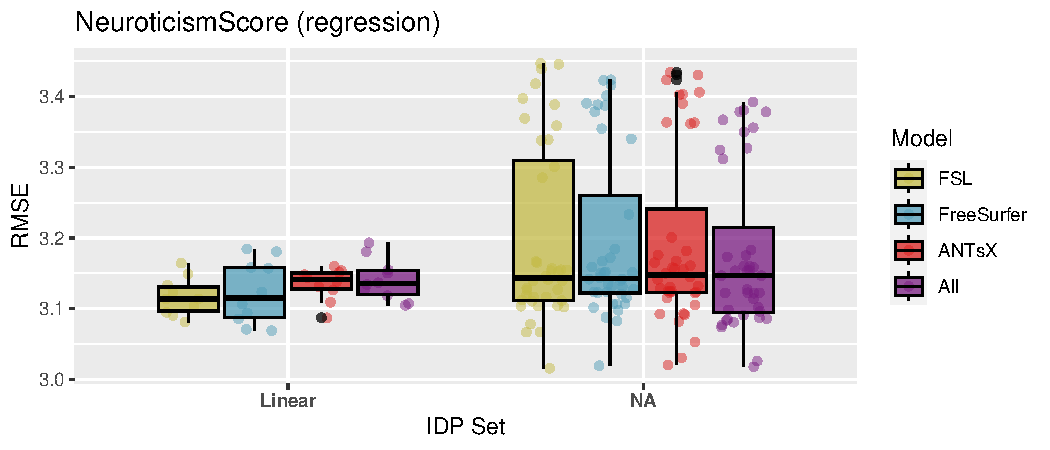
\includegraphics{/Users/ntustison/Documents/Academic/InProgress/ANTsXUKBB/Text/Figures/compare_predictions_NeuroticismScore.pdf}
\caption{NeuroticismScore}
\end{figure}

\hypertarget{feature-ranking-linear-2}{%
\subsection{Feature ranking: Linear}\label{feature-ranking-linear-2}}

\begin{table}

\caption{\label{tab:compare-predictions}NeuroticismScore}
\centering
\begin{tabular}[t]{lll}
\toprule
Package & Pipeline & Feature\\
\midrule
FSL & FAST & Volume of grey matter in Amygdala (left)\\
FSL & FAST & Volume of grey matter in Amygdala (right)\\
FSL & FAST & Volume of grey matter in Superior Frontal Gyrus (left)\\
ANTsX & Thickness & Right pericalcarine\\
ANTsX & Cortical & Right middle temporal volume\\
\addlinespace
FSL & FAST & Volume of grey matter in VI Cerebellum (vermis)\\
FreeSurfer & ASEG & Volume of CC-Posterior (whole brain)\\
FSL & FAST & Volume of grey matter in Frontal Operculum Cortex (left)\\
FSL & FAST & Volume of grey matter in Temporal Pole (left)\\
ANTsX & Thickness & Right postcentral\\
\addlinespace
ANTsX & Thickness & Left supramarginal\\
ANTsX & Cortical & Right isthmus cingulate volume\\
FSL & FAST & Volume of grey matter in Middle Frontal Gyrus (left)\\
ANTsX & Cereb & L\_VIIIA thickness\\
ANTsX & Region & Right middle temporal\\
\addlinespace
FreeSurfer & HippAmyg & Volume of Whole-hippocampus (right hemisphere)\\
FreeSurfer & Volume & Volume of medialorbitofrontal (left hemisphere)\\
FreeSurfer & Thickness & Mean thickness of superiorparietal (right hemisphere)\\
FreeSurfer & Volume & Volume of parstriangularis (right hemisphere)\\
FreeSurfer & Thickness & Mean thickness of parsopercularis (left hemisphere)\\
\addlinespace
FSL & FAST & Volume of grey matter in Caudate (right)\\
ANTsX & Region & Left posterior cingulate\\
ANTsX & DeepFLASH & Left aLEC\\
FSL & FAST & Volume of grey matter in Frontal Pole (right)\\
FreeSurfer & Volume & Volume of fusiform (left hemisphere)\\
\bottomrule
\end{tabular}
\end{table}

\begin{itemize}
\item
  FSL

  \begin{itemize}
  \item
    range: {[} 0.1497857 , 11.49945 {]}
  \item
    std: 1.249287
  \item
    skewness: 5.875585
  \end{itemize}
\item
  FreeSurfer

  \begin{itemize}
  \item
    range: {[} 0.1914575 , 3.135206 {]}
  \item
    std: 0.4852226
  \item
    skewness: 1.354637
  \end{itemize}
\item
  ANTsX

  \begin{itemize}
  \item
    range: {[} 0.1026427 , 3.387002 {]}
  \item
    std: 0.5902549
  \item
    skewness: 1.504382
  \end{itemize}
\end{itemize}

\hypertarget{package-based-ranking-top-10-features-2}{%
\subsubsection{Package-based ranking (top 10
features)}\label{package-based-ranking-top-10-features-2}}

\begin{itemize}
\item
  FSL: rank = 116 , imp = 43.61838
\item
  FreeSurfer: rank = 213 , imp = 23.50922
\item
  ANTsX: rank = 143 , imp = 27.62823
\end{itemize}

\hypertarget{package-based-ranking-top-25-features-2}{%
\subsubsection{Package-based ranking (top 25
features)}\label{package-based-ranking-top-25-features-2}}

\begin{itemize}
\item
  FSL: rank = 973 , imp = 69.36826
\item
  FreeSurfer: rank = 1130 , imp = 48.81682
\item
  ANTsX: rank = 842 , imp = 54.85405
\end{itemize}

\hypertarget{package-based-ranking-top-50-features-2}{%
\subsubsection{Package-based ranking (top 50
features)}\label{package-based-ranking-top-50-features-2}}

\begin{itemize}
\item
  FSL: rank = 4902 , imp = 99.63279
\item
  FreeSurfer: rank = 3959 , imp = 83.64052
\item
  ANTsX: rank = 3164 , imp = 91.80446
\end{itemize}

\clearpage

\hypertarget{numericmemory}{%
\section{NumericMemory}\label{numericmemory}}

\begin{figure}
\centering
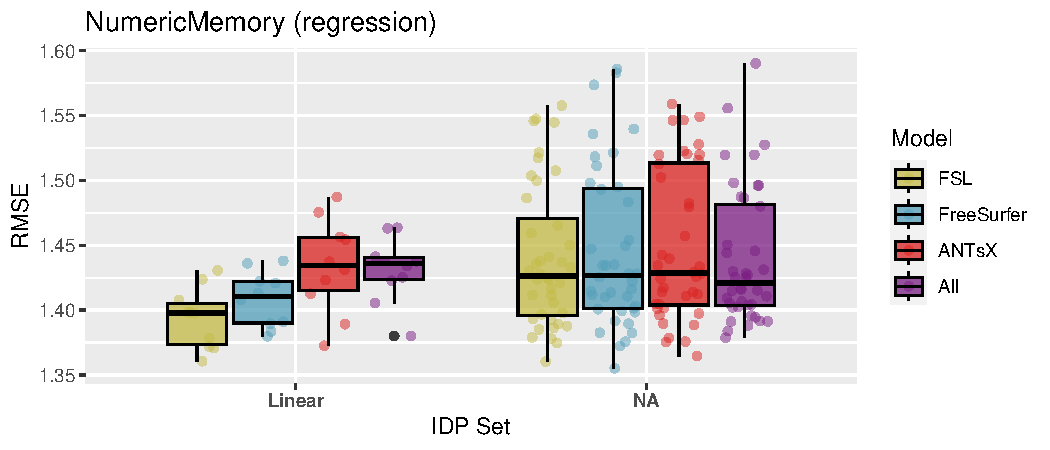
\includegraphics{/Users/ntustison/Documents/Academic/InProgress/ANTsXUKBB/Text/Figures/compare_predictions_NumericMemory.pdf}
\caption{NumericMemory}
\end{figure}

\hypertarget{feature-ranking-linear-3}{%
\subsection{Feature ranking: Linear}\label{feature-ranking-linear-3}}

\begin{table}

\caption{\label{tab:compare-predictions}NumericMemory}
\centering
\begin{tabular}[t]{lll}
\toprule
Package & Pipeline & Feature\\
\midrule
FSL & FAST & Volume of grey matter in Amygdala (left)\\
FSL & Other & Continuous    Volume of peripheral cortical grey matter\\
ANTsX & Thickness & Right lateral orbitofrontal\\
FSL & FAST & Volume of grey matter in Hippocampus (right)\\
FreeSurfer & ASEG & Volume of CSF (whole brain)\\
\addlinespace
FSL & FAST & Volume of grey matter in Precentral Gyrus (right)\\
FSL & FAST & Volume of grey matter in Middle Temporal Gyrus - temporooccipital part (right)\\
ANTsX & Cortical & Right isthmus cingulate volume\\
ANTsX & Region & Right isthmus cingulate\\
FreeSurfer & HippAmyg & Volume of Whole-hippocampus (left hemisphere)\\
\addlinespace
FreeSurfer & Thickness & Mean thickness of isthmuscingulate (left hemisphere)\\
ANTsX & DeepFLASH & Left subiculum\\
FSL & Other & Continuous    Volume of grey matter\\
ANTsX & Cereb & L\_I\_II thickness\\
FSL & FAST & Volume of grey matter in Crus I Cerebellum (vermis)\\
\addlinespace
ANTsX & Cortical & Left parahippocampal volume\\
FSL & Other & Continuous    Volume of peripheral cortical grey matter (normalised for head size)\\
FSL & FAST & Volume of grey matter in Intracalcarine Cortex (left)\\
ANTsX & Thickness & Right superior parietal\\
ANTsX & Cortical & Left caudal anterior cingulate volume\\
\addlinespace
ANTsX & Cortical & Right caudal anterior cingulate volume\\
ANTsX & DeepFLASH & Right MTL\\
ANTsX & Thickness & Right superior temporal\\
FreeSurfer & Thickness & Mean thickness of rostralanteriorcingulate (left hemisphere)\\
ANTsX & Region & Right lateral orbitofrontal\\
\bottomrule
\end{tabular}
\end{table}

\begin{itemize}
\item
  FSL

  \begin{itemize}
  \item
    range: {[} 0.09549313 , 4.647745 {]}
  \item
    std: 0.7300451
  \item
    skewness: 1.850753
  \end{itemize}
\item
  FreeSurfer

  \begin{itemize}
  \item
    range: {[} 0.1542513 , 2.957326 {]}
  \item
    std: 0.5181698
  \item
    skewness: 1.581697
  \end{itemize}
\item
  ANTsX

  \begin{itemize}
  \item
    range: {[} 0.1409571 , 3.140423 {]}
  \item
    std: 0.5994258
  \item
    skewness: 1.195387
  \end{itemize}
\end{itemize}

\hypertarget{package-based-ranking-top-10-features-3}{%
\subsubsection{Package-based ranking (top 10
features)}\label{package-based-ranking-top-10-features-3}}

\begin{itemize}
\item
  FSL: rank = 109 , imp = 29.89693
\item
  FreeSurfer: rank = 288 , imp = 22.55545
\item
  ANTsX: rank = 144 , imp = 26.20399
\end{itemize}

\hypertarget{package-based-ranking-top-25-features-3}{%
\subsubsection{Package-based ranking (top 25
features)}\label{package-based-ranking-top-25-features-3}}

\begin{itemize}
\item
  FSL: rank = 955 , imp = 57.76288
\item
  FreeSurfer: rank = 1238 , imp = 49.30908
\item
  ANTsX: rank = 755 , imp = 57.06385
\end{itemize}

\hypertarget{package-based-ranking-top-50-features-3}{%
\subsubsection{Package-based ranking (top 50
features)}\label{package-based-ranking-top-50-features-3}}

\begin{itemize}
\item
  FSL: rank = 4439 , imp = 90.58995
\item
  FreeSurfer: rank = 4467 , imp = 83.32317
\item
  ANTsX: rank = 2904 , imp = 97.12109
\end{itemize}

\clearpage

\hypertarget{bmi}{%
\section{BMI}\label{bmi}}

\begin{figure}
\centering
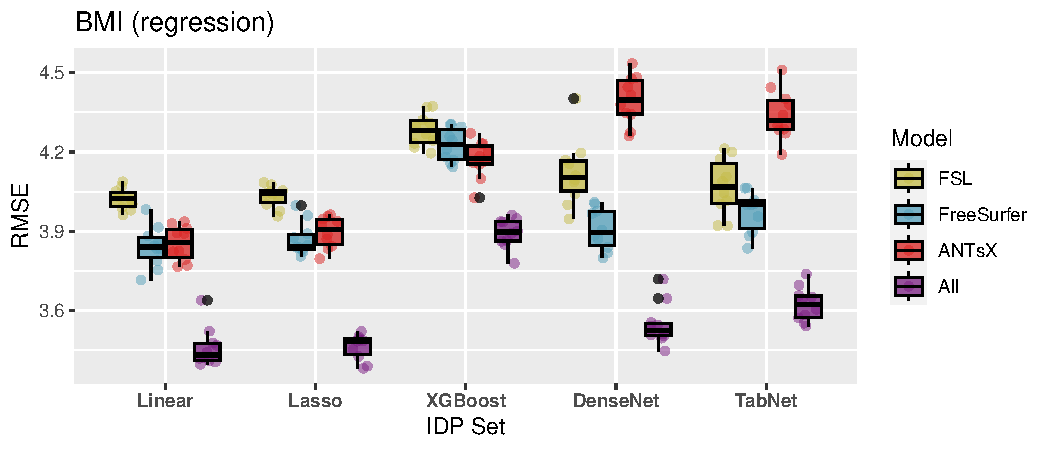
\includegraphics{/Users/ntustison/Documents/Academic/InProgress/ANTsXUKBB/Text/Figures/compare_predictions_BMI.pdf}
\caption{BMI}
\end{figure}

\hypertarget{feature-ranking-linear-4}{%
\subsection{Feature ranking: Linear}\label{feature-ranking-linear-4}}

\begin{table}

\caption{\label{tab:compare-predictions}BMI}
\centering
\begin{tabular}[t]{lll}
\toprule
Package & Pipeline & Feature\\
\midrule
ANTsX & Thickness & Left paracentral\\
FSL & FAST & Volume of grey matter in Amygdala (left)\\
FreeSurfer & ASEG & Volume of Cerebellum-White-Matter (right hemisphere)\\
ANTsX & Cereb & CerebellarGrayMatter volume\\
FreeSurfer & ASEG & Volume of Cerebellum-White-Matter (left hemisphere)\\
\addlinespace
ANTsX & Thickness & Left lingual\\
FreeSurfer & ASEG & Volume of EstimatedTotalIntraCranial (whole brain)\\
ANTsX & Atropos & BrainStem\\
FSL & Other & Continuous    Volume of peripheral cortical grey matter (normalised for head size)\\
FSL & FAST & Volume of grey matter in Occipital Fusiform Gyrus (right)\\
\addlinespace
FSL & FAST & Volume of grey matter in Lateral Occipital Cortex - superior division (right)\\
FSL & FAST & Volume of grey matter in Amygdala (right)\\
FSL & FAST & Volume of grey matter in Lingual Gyrus (right)\\
FreeSurfer & ASEG & Volume of VentralDC (right hemisphere)\\
FreeSurfer & ASEG & Volume of SupraTentorialNotVent (whole brain)\\
\addlinespace
FSL & FAST & Volume of grey matter in Caudate (left)\\
FreeSurfer & Thickness & Mean thickness of superiorfrontal (left hemisphere)\\
FSL & FAST & Volume of grey matter in Cuneal Cortex (left)\\
FSL & FAST & Volume of grey matter in VIIIa Cerebellum (left)\\
ANTsX & Region & Left thalamus proper\\
\addlinespace
FSL & FAST & Volume of grey matter in Pallidum (right)\\
FSL & FAST & Volume of grey matter in IX Cerebellum (right)\\
FreeSurfer & Volume & Volume of transversetemporal (right hemisphere)\\
FSL & FIRST & Volume of caudate (left)\\
FreeSurfer & Volume & Volume of isthmuscingulate (right hemisphere)\\
\bottomrule
\end{tabular}
\end{table}

\begin{itemize}
\item
  FSL

  \begin{itemize}
  \item
    range: {[} 0.1562628 , 12.46823 {]}
  \item
    std: 2.429514
  \item
    skewness: 1.476122
  \end{itemize}
\item
  FreeSurfer

  \begin{itemize}
  \item
    range: {[} 0.159632 , 12.3667 {]}
  \item
    std: 2.219477
  \item
    skewness: 1.776937
  \end{itemize}
\item
  ANTsX

  \begin{itemize}
  \item
    range: {[} 0.1637263 , 12.64787 {]}
  \item
    std: 1.924288
  \item
    skewness: 2.005405
  \end{itemize}
\end{itemize}

\hypertarget{package-based-ranking-top-10-features-4}{%
\subsubsection{Package-based ranking (top 10
features)}\label{package-based-ranking-top-10-features-4}}

\begin{itemize}
\item
  FSL: rank = 131 , imp = 94.45128
\item
  FreeSurfer: rank = 164 , imp = 91.74847
\item
  ANTsX: rank = 210 , imp = 88.12971
\end{itemize}

\hypertarget{package-based-ranking-top-25-features-4}{%
\subsubsection{Package-based ranking (top 25
features)}\label{package-based-ranking-top-25-features-4}}

\begin{itemize}
\item
  FSL: rank = 923 , imp = 187.4333
\item
  FreeSurfer: rank = 796 , imp = 188.4521
\item
  ANTsX: rank = 1220 , imp = 172.7291
\end{itemize}

\hypertarget{package-based-ranking-top-50-features-4}{%
\subsubsection{Package-based ranking (top 50
features)}\label{package-based-ranking-top-50-features-4}}

\begin{itemize}
\item
  FSL: rank = 4453 , imp = 284.1735
\item
  FreeSurfer: rank = 3170 , imp = 307.6056
\item
  ANTsX: rank = 4106 , imp = 277.511
\end{itemize}

\clearpage

\hypertarget{townsenddeprivationindex}{%
\section{TownsendDeprivationIndex}\label{townsenddeprivationindex}}

\begin{figure}
\centering
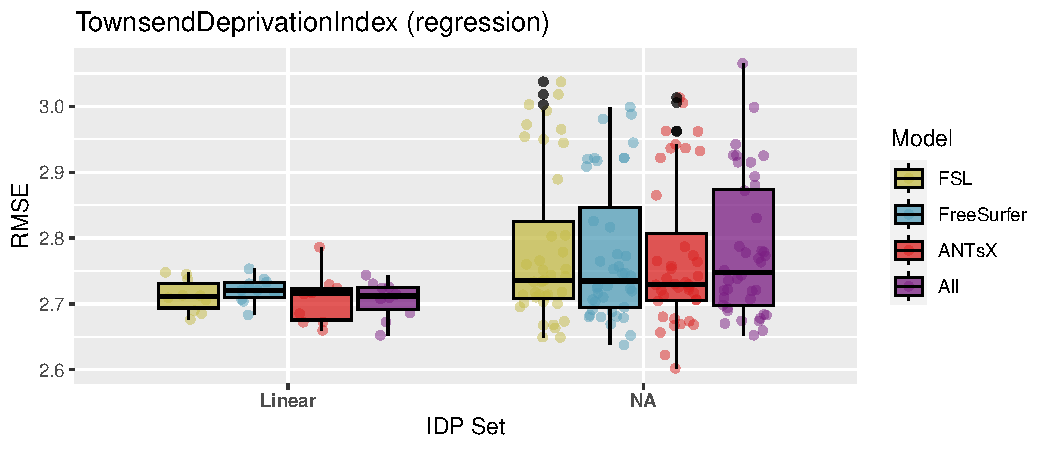
\includegraphics{/Users/ntustison/Documents/Academic/InProgress/ANTsXUKBB/Text/Figures/compare_predictions_TownsendDeprivationIndex.pdf}
\caption{TownsendDeprivationIndex}
\end{figure}

\hypertarget{feature-ranking-linear-5}{%
\subsection{Feature ranking: Linear}\label{feature-ranking-linear-5}}

\begin{table}

\caption{\label{tab:compare-predictions}TownsendDeprivationIndex}
\centering
\begin{tabular}[t]{lll}
\toprule
Package & Pipeline & Feature\\
\midrule
FSL & FAST & Volume of grey matter in Amygdala (left)\\
FSL & Other & Continuous    Volume of peripheral cortical grey matter\\
FSL & FAST & Volume of grey matter in Heschl's Gyrus (includes H1 and H2) (left)\\
FSL & Other & Continuous    Volume of ventricular cerebrospinal fluid\\
FSL & Other & Continuous    Volume of ventricular cerebrospinal fluid (normalised for head size)\\
\addlinespace
FreeSurfer & ASEG & Volume of SupraTentorial (whole brain)\\
FreeSurfer & ASEG & Volume of VentralDC (left hemisphere)\\
FSL & FAST & Volume of grey matter in Heschl's Gyrus (includes H1 and H2) (right)\\
ANTsX & SYSU WMH & Left cerebellum\\
FreeSurfer & ASEG & Volume of TotalGray (whole brain)\\
\addlinespace
FSL & FAST & Volume of grey matter in Superior Parietal Lobule (right)\\
FreeSurfer & Thickness & Mean thickness of superiorfrontal (right hemisphere)\\
ANTsX & Cereb & CerebellarGrayMatter volume\\
ANTsX & Cereb & L\_III volume\\
ANTsX & Region & Right caudal anterior cingulate\\
\addlinespace
ANTsX & Cortical & Left insula volume\\
FreeSurfer & ASEG & Volume of SupraTentorialNotVent (whole brain)\\
FSL & FAST & Volume of grey matter in Thalamus (left)\\
ANTsX & Thickness & Left superior parietal\\
FSL & FAST & Volume of grey matter in Inferior Temporal Gyrus - temporooccipital part (left)\\
\addlinespace
FSL & FAST & Volume of grey matter in Frontal Pole (right)\\
FSL & FAST & Volume of grey matter in Planum Temporale (left)\\
ANTsX & Cereb & R\_X volume\\
FreeSurfer & Thickness & Mean thickness of superiortemporal (left hemisphere)\\
FSL & FAST & Volume of grey matter in Occipital Fusiform Gyrus (left)\\
\bottomrule
\end{tabular}
\end{table}

\begin{itemize}
\item
  FSL

  \begin{itemize}
  \item
    range: {[} 0.139757 , 12.48687 {]}
  \item
    std: 1.248796
  \item
    skewness: 4.841903
  \end{itemize}
\item
  FreeSurfer

  \begin{itemize}
  \item
    range: {[} 0.1699931 , 3.64896 {]}
  \item
    std: 0.6524566
  \item
    skewness: 1.065419
  \end{itemize}
\item
  ANTsX

  \begin{itemize}
  \item
    range: {[} 0.158075 , 3.297345 {]}
  \item
    std: 0.6863873
  \item
    skewness: 1.076649
  \end{itemize}
\end{itemize}

\hypertarget{package-based-ranking-top-10-features-5}{%
\subsubsection{Package-based ranking (top 10
features)}\label{package-based-ranking-top-10-features-5}}

\begin{itemize}
\item
  FSL: rank = 93 , imp = 44.74012
\item
  FreeSurfer: rank = 233 , imp = 29.08779
\item
  ANTsX: rank = 193 , imp = 29.35449
\end{itemize}

\hypertarget{package-based-ranking-top-25-features-5}{%
\subsubsection{Package-based ranking (top 25
features)}\label{package-based-ranking-top-25-features-5}}

\begin{itemize}
\item
  FSL: rank = 763 , imp = 80.4624
\item
  FreeSurfer: rank = 1274 , imp = 60.26641
\item
  ANTsX: rank = 891 , imp = 64.35683
\end{itemize}

\hypertarget{package-based-ranking-top-50-features-5}{%
\subsubsection{Package-based ranking (top 50
features)}\label{package-based-ranking-top-50-features-5}}

\begin{itemize}
\item
  FSL: rank = 4128 , imp = 121.9611
\item
  FreeSurfer: rank = 4139 , imp = 104.0827
\item
  ANTsX: rank = 3281 , imp = 111.1481
\end{itemize}

\clearpage

\hypertarget{geneticsex}{%
\section{GeneticSex}\label{geneticsex}}

\begin{figure}
\centering
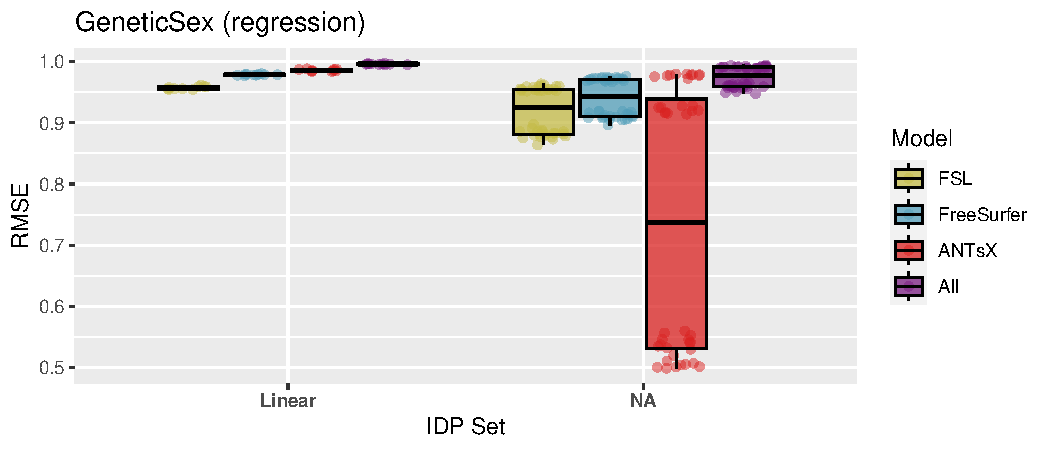
\includegraphics{/Users/ntustison/Documents/Academic/InProgress/ANTsXUKBB/Text/Figures/compare_predictions_GeneticSex.pdf}
\caption{GeneticSex}
\end{figure}

\hypertarget{feature-ranking-linear-6}{%
\subsection{Feature ranking: Linear}\label{feature-ranking-linear-6}}

\begin{table}

\caption{\label{tab:compare-predictions}GeneticSex}
\centering
\begin{tabular}[t]{lll}
\toprule
Package & Pipeline & Feature\\
\midrule
ANTsX & Atropos & DeepGrayMatter\\
FreeSurfer & HippAmyg & Volume of AV (right hemisphere)\\
FreeSurfer & ASEG & Volume of VentralDC (right hemisphere)\\
FreeSurfer & ASEG & Volume of CerebralWhiteMatter (left hemisphere)\\
ANTsX & Region & Left thalamus proper\\
\addlinespace
FreeSurfer & ASEG & Volume of CerebralWhiteMatter (right hemisphere)\\
FreeSurfer & ASEG & Volume of Cortex (right hemisphere)\\
FreeSurfer & ASEG & Volume of Cortex (left hemisphere)\\
FreeSurfer & ASEG & Volume of CC-Central (whole brain)\\
FSL & FIRST & Volume of accumbens (left)\\
\addlinespace
FSL & FAST & Volume of grey matter in Lateral Occipital Cortex - superior division (left)\\
ANTsX & Cortical & Right lateral occipital volume\\
FSL & FAST & Volume of grey matter in Frontal Medial Cortex (left)\\
ANTsX & Region & Right caudate\\
-- & -- & NA\\
\addlinespace
FreeSurfer & Thickness & Mean thickness of paracentral (right hemisphere)\\
FreeSurfer & Volume & Volume of transversetemporal (left hemisphere)\\
ANTsX & Cereb & R\_IX thickness\\
ANTsX & Cortical & Left parahippocampal volume\\
ANTsX & Cereb & R\_VIIB thickness\\
\addlinespace
FreeSurfer & HippAmyg & Volume of AV (left hemisphere)\\
ANTsX & Cortical & Right superior parietal volume\\
ANTsX & Cereb & CerebellarWhiteMatter volume\\
ANTsX & Region & Right inferior parietal\\
FSL & FAST & Volume of grey matter in Intracalcarine Cortex (right)\\
\bottomrule
\end{tabular}
\end{table}

\begin{itemize}
\item
  FSL

  \begin{itemize}
  \item
    range: {[} NA , NA {]}
  \item
    std: NA
  \item
    skewness: NA
  \end{itemize}
\item
  FreeSurfer

  \begin{itemize}
  \item
    range: {[} 0.1737775 , 10.24362 {]}
  \item
    std: 1.567378
  \item
    skewness: 2.222905
  \end{itemize}
\item
  ANTsX

  \begin{itemize}
  \item
    range: {[} 0.1889526 , 10.59129 {]}
  \item
    std: 1.589695
  \item
    skewness: 1.313573
  \end{itemize}
\end{itemize}

\hypertarget{package-based-ranking-top-10-features-6}{%
\subsubsection{Package-based ranking (top 10
features)}\label{package-based-ranking-top-10-features-6}}

\begin{itemize}
\item
  FSL: rank = 305 , imp = 56.68502
\item
  FreeSurfer: rank = 93 , imp = 74.87624
\item
  ANTsX: rank = 158 , imp = 66.55404
\end{itemize}

\hypertarget{package-based-ranking-top-25-features-6}{%
\subsubsection{Package-based ranking (top 25
features)}\label{package-based-ranking-top-25-features-6}}

\begin{itemize}
\item
  FSL: rank = 1498 , imp = 117.6986
\item
  FreeSurfer: rank = 868 , imp = 146.3458
\item
  ANTsX: rank = 781 , imp = 142.2774
\end{itemize}

\hypertarget{package-based-ranking-top-50-features-6}{%
\subsubsection{Package-based ranking (top 50
features)}\label{package-based-ranking-top-50-features-6}}

\begin{itemize}
\item
  FSL: rank = 5321 , imp = 194.8791
\item
  FreeSurfer: rank = 4226 , imp = 228.9607
\item
  ANTsX: rank = 2835 , imp = 243.0013
\end{itemize}

\clearpage

\hypertarget{hearing}{%
\section{Hearing}\label{hearing}}

\begin{figure}
\centering
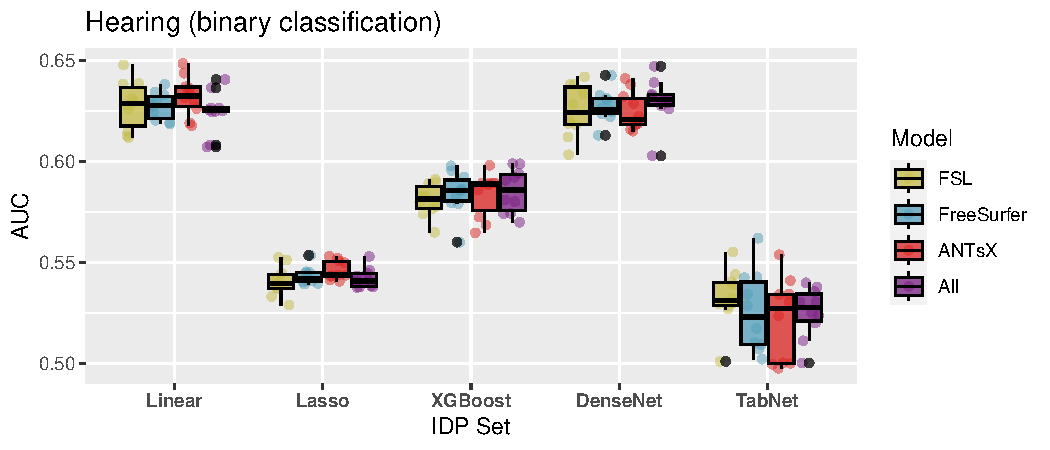
\includegraphics{/Users/ntustison/Documents/Academic/InProgress/ANTsXUKBB/Text/Figures/compare_predictions_Hearing.pdf}
\caption{Hearing}
\end{figure}

\hypertarget{feature-ranking-linear-7}{%
\subsection{Feature ranking: Linear}\label{feature-ranking-linear-7}}

\begin{table}

\caption{\label{tab:compare-predictions}Hearing}
\centering
\begin{tabular}[t]{lll}
\toprule
Package & Pipeline & Feature\\
\midrule
FSL & FAST & Volume of grey matter in Amygdala (left)\\
FSL & FAST & Volume of grey matter in Amygdala (right)\\
ANTsX & Thickness & Right lingual\\
ANTsX & Cereb & L\_IX volume\\
ANTsX & DeepFLASH & Left aLEC\\
\addlinespace
ANTsX & Thickness & Left transverse temporal\\
FreeSurfer & Volume & Volume of caudalanteriorcingulate (left hemisphere)\\
FSL & FAST & Volume of grey matter in X Cerebellum (right)\\
FreeSurfer & Volume & Volume of medialorbitofrontal (left hemisphere)\\
FSL & FAST & Volume of grey matter in Temporal Fusiform Cortex - posterior division (left)\\
\addlinespace
FreeSurfer & Thickness & Mean thickness of posteriorcingulate (right hemisphere)\\
FSL & Other & Continuous    Volume of grey matter\\
FreeSurfer & Volume & Volume of paracentral (left hemisphere)\\
ANTsX & Region & Right thalamus proper\\
ANTsX & Cereb & L\_Crus\_I volume\\
\addlinespace
ANTsX & Cereb & L\_I\_II volume\\
FreeSurfer & Volume & Volume of inferiorparietal (left hemisphere)\\
FreeSurfer & Thickness & Mean thickness of inferiorparietal (left hemisphere)\\
ANTsX & Cereb & R\_VI volume\\
ANTsX & Region & Right caudate\\
\addlinespace
FSL & FAST & Volume of grey matter in VI Cerebellum (right)\\
FSL & FAST & Volume of grey matter in Parahippocampal Gyrus - posterior division (left)\\
FSL & FAST & Volume of grey matter in Middle Temporal Gyrus - temporooccipital part (right)\\
ANTsX & Region & Right middle temporal\\
ANTsX & Cereb & L\_Crus\_II volume\\
\bottomrule
\end{tabular}
\end{table}

\begin{itemize}
\item
  FSL

  \begin{itemize}
  \item
    range: {[} 0.1400707 , 15.84752 {]}
  \item
    std: 1.370073
  \item
    skewness: 7.933981
  \end{itemize}
\item
  FreeSurfer

  \begin{itemize}
  \item
    range: {[} 0.1609316 , 3.033436 {]}
  \item
    std: 0.6188603
  \item
    skewness: 1.169872
  \end{itemize}
\item
  ANTsX

  \begin{itemize}
  \item
    range: {[} 0.09976114 , 3.424184 {]}
  \item
    std: 0.6634497
  \item
    skewness: 1.186676
  \end{itemize}
\end{itemize}

\hypertarget{package-based-ranking-top-10-features-7}{%
\subsubsection{Package-based ranking (top 10
features)}\label{package-based-ranking-top-10-features-7}}

\begin{itemize}
\item
  FSL: rank = 157 , imp = 41.91777
\item
  FreeSurfer: rank = 195 , imp = 26.48697
\item
  ANTsX: rank = 126 , imp = 28.82698
\end{itemize}

\hypertarget{package-based-ranking-top-25-features-7}{%
\subsubsection{Package-based ranking (top 25
features)}\label{package-based-ranking-top-25-features-7}}

\begin{itemize}
\item
  FSL: rank = 1280 , imp = 70.92944
\item
  FreeSurfer: rank = 933 , imp = 59.54118
\item
  ANTsX: rank = 820 , imp = 62.38052
\end{itemize}

\hypertarget{package-based-ranking-top-50-features-7}{%
\subsubsection{Package-based ranking (top 50
features)}\label{package-based-ranking-top-50-features-7}}

\begin{itemize}
\item
  FSL: rank = 5838 , imp = 103.0179
\item
  FreeSurfer: rank = 3514 , imp = 101.4115
\item
  ANTsX: rank = 3120 , imp = 106.2714
\end{itemize}

\clearpage

\hypertarget{risktaking}{%
\section{RiskTaking}\label{risktaking}}

\begin{figure}
\centering
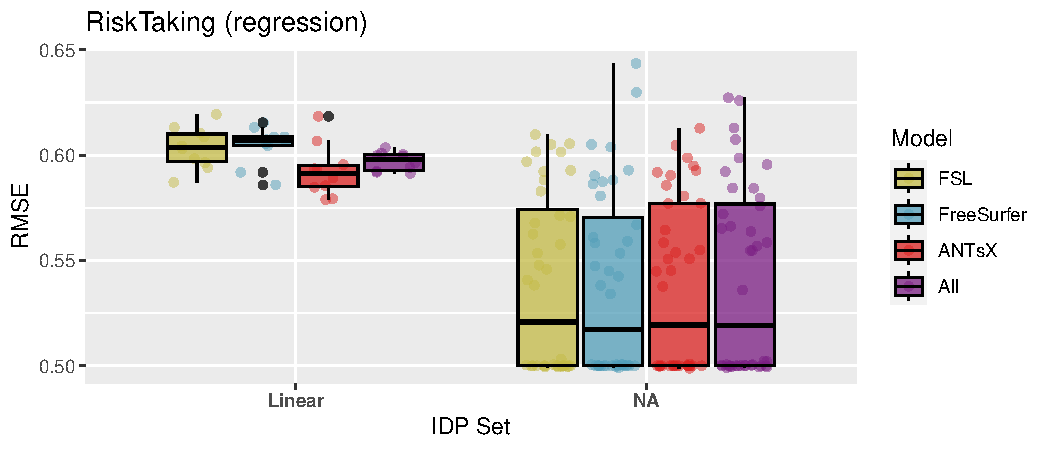
\includegraphics{/Users/ntustison/Documents/Academic/InProgress/ANTsXUKBB/Text/Figures/compare_predictions_RiskTaking.pdf}
\caption{RiskTaking}
\end{figure}

\hypertarget{feature-ranking-linear-8}{%
\subsection{Feature ranking: Linear}\label{feature-ranking-linear-8}}

\begin{table}

\caption{\label{tab:compare-predictions}RiskTaking}
\centering
\begin{tabular}[t]{lll}
\toprule
Package & Pipeline & Feature\\
\midrule
FSL & FAST & Volume of grey matter in Amygdala (right)\\
FSL & FAST & Volume of grey matter in Amygdala (left)\\
FreeSurfer & ASEG & Volume of BrainSeg (whole brain)\\
FSL & FAST & Volume of grey matter in Frontal Orbital Cortex (left)\\
FreeSurfer & Thickness & Mean thickness of parsorbitalis (left hemisphere)\\
\addlinespace
FreeSurfer & HippAmyg & Volume of CL (left hemisphere)\\
FreeSurfer & HippAmyg & Volume of Hippocampal-tail (left hemisphere)\\
ANTsX & Thickness & Left caudal anterior cingulate\\
FreeSurfer & HippAmyg & Volume of parasubiculum (left hemisphere)\\
FreeSurfer & HippAmyg & Volume of presubiculum-body (left hemisphere)\\
\addlinespace
FreeSurfer & HippAmyg & Volume of CA3-body (left hemisphere)\\
FreeSurfer & HippAmyg & Volume of CA4-body (left hemisphere)\\
FreeSurfer & HippAmyg & Volume of subiculum-body (left hemisphere)\\
FreeSurfer & HippAmyg & Volume of HATA (left hemisphere)\\
FSL & FAST & Volume of grey matter in Temporal Fusiform Cortex - anterior division (left)\\
\addlinespace
FSL & FAST & Volume of grey matter in Intracalcarine Cortex (left)\\
FreeSurfer & Thickness & Mean thickness of lateralorbitofrontal (right hemisphere)\\
ANTsX & DeepFLASH & Right perirhinal\\
ANTsX & Cortical & Right pericalcarine volume\\
ANTsX & DeepFLASH & Right MTL\\
\addlinespace
ANTsX & Region & Right pericalcarine\\
FreeSurfer & HippAmyg & Volume of AV (right hemisphere)\\
FreeSurfer & ASEG & Volume of Amygdala (left hemisphere)\\
FreeSurfer & ASEG & Volume of TotalGray (whole brain)\\
FreeSurfer & Thickness & Mean thickness of entorhinal (left hemisphere)\\
\bottomrule
\end{tabular}
\end{table}

\begin{itemize}
\item
  FSL

  \begin{itemize}
  \item
    range: {[} 0.1795269 , 10.14113 {]}
  \item
    std: 0.9923587
  \item
    skewness: 5.553114
  \end{itemize}
\item
  FreeSurfer

  \begin{itemize}
  \item
    range: {[} 0.1836498 , 3.657539 {]}
  \item
    std: 0.6951129
  \item
    skewness: 0.6690752
  \end{itemize}
\item
  ANTsX

  \begin{itemize}
  \item
    range: {[} 0.1370474 , 2.901573 {]}
  \item
    std: 0.6013431
  \item
    skewness: 0.9711023
  \end{itemize}
\end{itemize}

\hypertarget{package-based-ranking-top-10-features-8}{%
\subsubsection{Package-based ranking (top 10
features)}\label{package-based-ranking-top-10-features-8}}

\begin{itemize}
\item
  FSL: rank = 261 , imp = 34.88583
\item
  FreeSurfer: rank = 90 , imp = 30.03523
\item
  ANTsX: rank = 250 , imp = 25.28125
\end{itemize}

\hypertarget{package-based-ranking-top-25-features-8}{%
\subsubsection{Package-based ranking (top 25
features)}\label{package-based-ranking-top-25-features-8}}

\begin{itemize}
\item
  FSL: rank = 2255 , imp = 59.555
\item
  FreeSurfer: rank = 552 , imp = 65.86192
\item
  ANTsX: rank = 1073 , imp = 55.84686
\end{itemize}

\hypertarget{package-based-ranking-top-50-features-8}{%
\subsubsection{Package-based ranking (top 50
features)}\label{package-based-ranking-top-50-features-8}}

\begin{itemize}
\item
  FSL: rank = 8514 , imp = 90.72164
\item
  FreeSurfer: rank = 2525 , imp = 111.9594
\item
  ANTsX: rank = 3945 , imp = 97.4797
\end{itemize}

\clearpage

\hypertarget{samesexintercourse}{%
\section{SameSexIntercourse}\label{samesexintercourse}}

\begin{figure}
\centering
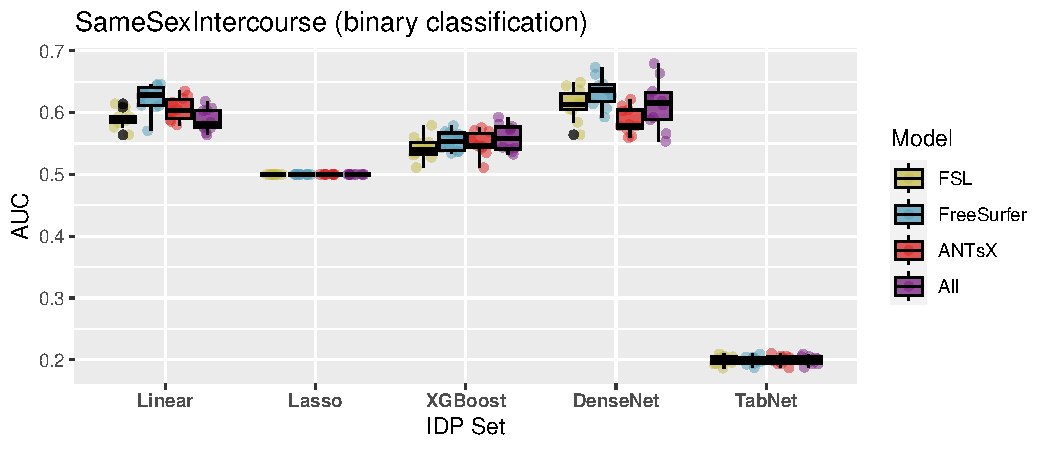
\includegraphics{/Users/ntustison/Documents/Academic/InProgress/ANTsXUKBB/Text/Figures/compare_predictions_SameSexIntercourse.pdf}
\caption{SameSexIntercourse}
\end{figure}

\hypertarget{feature-ranking-linear-9}{%
\subsection{Feature ranking: Linear}\label{feature-ranking-linear-9}}

\begin{table}

\caption{\label{tab:compare-predictions}SameSexIntercourse}
\centering
\begin{tabular}[t]{lll}
\toprule
Package & Pipeline & Feature\\
\midrule
FSL & FAST & Volume of grey matter in Amygdala (left)\\
FreeSurfer & ASEG & Volume of CC-Mid-Anterior (whole brain)\\
ANTsX & SYSU WMH & Left brain stem\\
ANTsX & Region & Left lingual\\
ANTsX & Region & Right ventral DC\\
\addlinespace
ANTsX & Region & CSF\\
FreeSurfer & ASEG & Volume of Optic-Chiasm (whole brain)\\
ANTsX & Thickness & Left rostral anterior cingulate\\
ANTsX & Region & Cerebellar vermal lobules VI VII\\
ANTsX & Cortical & Left lingual volume\\
\addlinespace
FSL & FAST & Volume of grey matter in Planum Polare (left)\\
ANTsX & Thickness & Right lateral orbitofrontal\\
ANTsX & Thickness & Right lateral occipital\\
ANTsX & Region & Left pars triangularis\\
ANTsX & Cortical & Left rostral anterior cingulate volume\\
\addlinespace
FreeSurfer & ASEG & Volume of non-WM-hypointensities (whole brain)\\
FSL & Other & Continuous    Volume of peripheral cortical grey matter (normalised for head size)\\
ANTsX & Cereb & R\_IV thickness\\
FreeSurfer & ASEG & Volume of Pallidum (left hemisphere)\\
FreeSurfer & ASEG & Volume of Lateral-Ventricle (left hemisphere)\\
\addlinespace
FSL & FAST & Volume of grey matter in Superior Frontal Gyrus (right)\\
FSL & FAST & Volume of grey matter in Frontal Medial Cortex (left)\\
ANTsX & Region & Left putamen\\
ANTsX & Thickness & Left lateral occipital\\
ANTsX & Thickness & Right superior frontal\\
\bottomrule
\end{tabular}
\end{table}

\begin{itemize}
\item
  FSL

  \begin{itemize}
  \item
    range: {[} 0.09777208 , 8.065794 {]}
  \item
    std: 0.7925432
  \item
    skewness: 4.774372
  \end{itemize}
\item
  FreeSurfer

  \begin{itemize}
  \item
    range: {[} 0.177841 , 3.047648 {]}
  \item
    std: 0.4620206
  \item
    skewness: 1.247426
  \end{itemize}
\item
  ANTsX

  \begin{itemize}
  \item
    range: {[} 0.1354761 , 2.923016 {]}
  \item
    std: 0.591493
  \item
    skewness: 1.252716
  \end{itemize}
\end{itemize}

\hypertarget{package-based-ranking-top-10-features-9}{%
\subsubsection{Package-based ranking (top 10
features)}\label{package-based-ranking-top-10-features-9}}

\begin{itemize}
\item
  FSL: rank = 234 , imp = 27.48743
\item
  FreeSurfer: rank = 329 , imp = 21.42504
\item
  ANTsX: rank = 84 , imp = 25.76776
\end{itemize}

\hypertarget{package-based-ranking-top-25-features-9}{%
\subsubsection{Package-based ranking (top 25
features)}\label{package-based-ranking-top-25-features-9}}

\begin{itemize}
\item
  FSL: rank = 1130 , imp = 53.00098
\item
  FreeSurfer: rank = 1717 , imp = 43.43501
\item
  ANTsX: rank = 543 , imp = 56.88152
\end{itemize}

\hypertarget{package-based-ranking-top-50-features-9}{%
\subsubsection{Package-based ranking (top 50
features)}\label{package-based-ranking-top-50-features-9}}

\begin{itemize}
\item
  FSL: rank = 4806 , imp = 84.5719
\item
  FreeSurfer: rank = 5014 , imp = 76.10665
\item
  ANTsX: rank = 2298 , imp = 97.2722
\end{itemize}

\clearpage

\hypertarget{smoking}{%
\section{Smoking}\label{smoking}}

\begin{figure}
\centering
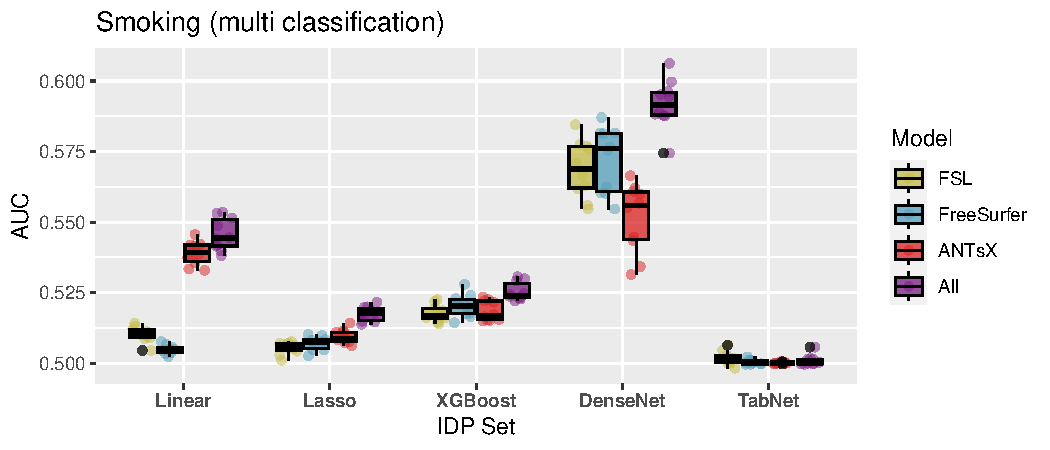
\includegraphics{/Users/ntustison/Documents/Academic/InProgress/ANTsXUKBB/Text/Figures/compare_predictions_Smoking.pdf}
\caption{Smoking}
\end{figure}

\hypertarget{feature-ranking-linear-10}{%
\subsection{Feature ranking: Linear}\label{feature-ranking-linear-10}}

\begin{table}

\caption{\label{tab:compare-predictions}Smoking}
\centering
\begin{tabular}[t]{lll}
\toprule
Package & Pipeline & Feature\\
\midrule
FreeSurfer & ASEG & Volume of CC-Central (whole brain)\\
FreeSurfer & ASEG & Volume of BrainSegNotVentSurf (whole brain)\\
FreeSurfer & ASEG & Volume of VentralDC (right hemisphere)\\
FreeSurfer & ASEG & Volume of Cortex (right hemisphere)\\
FreeSurfer & ASEG & Volume of Cortex (left hemisphere)\\
\addlinespace
FreeSurfer & ASEG & Volume of CC-Anterior (whole brain)\\
FreeSurfer & ASEG & Volume of Optic-Chiasm (whole brain)\\
FreeSurfer & ASEG & Volume of SupraTentorialNotVent (whole brain)\\
FreeSurfer & ASEG & Volume of Thalamus-Proper (right hemisphere)\\
FSL & Other & Continuous    Volume of brain stem + 4th ventricle\\
\addlinespace
FreeSurfer & ASEG & Volume of Pallidum (left hemisphere)\\
-- & -- & NA\\
FreeSurfer & ASEG & Volume of CerebralWhiteMatter (left hemisphere)\\
FreeSurfer & Thickness & Mean thickness of caudalanteriorcingulate (left hemisphere)\\
ANTsX & Cortical & Left superior frontal volume\\
\addlinespace
FSL & Other & Continuous    Volume of ventricular cerebrospinal fluid\\
FreeSurfer & ASEG & Volume of EstimatedTotalIntraCranial (whole brain)\\
FreeSurfer & ASEG & Volume of Thalamus-Proper (left hemisphere)\\
ANTsX & Atropos & BrainStem\\
FSL & Other & Continuous    Volume of brain = grey+white matter (normalised for head size)\\
\addlinespace
ANTsX & Atropos & WhiteMatter\\
FreeSurfer & ASEG & Volume of CerebralWhiteMatter (right hemisphere)\\
FSL & Other & Continuous    Volume of grey matter\\
FSL & Other & Continuous    Volume of white matter\\
FSL & Other & Continuous    Volume of grey matter (normalised for head size)\\
\bottomrule
\end{tabular}
\end{table}

\begin{itemize}
\item
  FSL

  \begin{itemize}
  \item
    range: {[} 0.0000000004780733 , 0.04568151 {]}
  \item
    std: 0.005543492
  \item
    skewness: 4.73262
  \end{itemize}
\item
  FreeSurfer

  \begin{itemize}
  \item
    range: {[} 0 , 0.3827131 {]}
  \item
    std: 0.03270468
  \item
    skewness: 8.254631
  \end{itemize}
\item
  ANTsX

  \begin{itemize}
  \item
    range: {[} 0.00000000000009869648 , 0.02975863 {]}
  \item
    std: 0.004373508
  \item
    skewness: 3.083098
  \end{itemize}
\end{itemize}

\hypertarget{package-based-ranking-top-10-features-10}{%
\subsubsection{Package-based ranking (top 10
features)}\label{package-based-ranking-top-10-features-10}}

\begin{itemize}
\item
  FSL: rank = 300 , imp = 0.2110577
\item
  FreeSurfer: rank = 56 , imp = 1.461918
\item
  ANTsX: rank = 262 , imp = 0.2076409
\end{itemize}

\hypertarget{package-based-ranking-top-25-features-10}{%
\subsubsection{Package-based ranking (top 25
features)}\label{package-based-ranking-top-25-features-10}}

\begin{itemize}
\item
  FSL: rank = 1886 , imp = 0.2870485
\item
  FreeSurfer: rank = 607 , imp = 1.719945
\item
  ANTsX: rank = 977 , imp = 0.3637066
\end{itemize}

\hypertarget{package-based-ranking-top-50-features-10}{%
\subsubsection{Package-based ranking (top 50
features)}\label{package-based-ranking-top-50-features-10}}

\begin{itemize}
\item
  FSL: rank = 6707 , imp = 0.3520102
\item
  FreeSurfer: rank = 3375 , imp = 1.842075
\item
  ANTsX: rank = 3086 , imp = 0.5167613
\end{itemize}

\clearpage

\hypertarget{alcohol}{%
\section{Alcohol}\label{alcohol}}

\begin{figure}
\centering
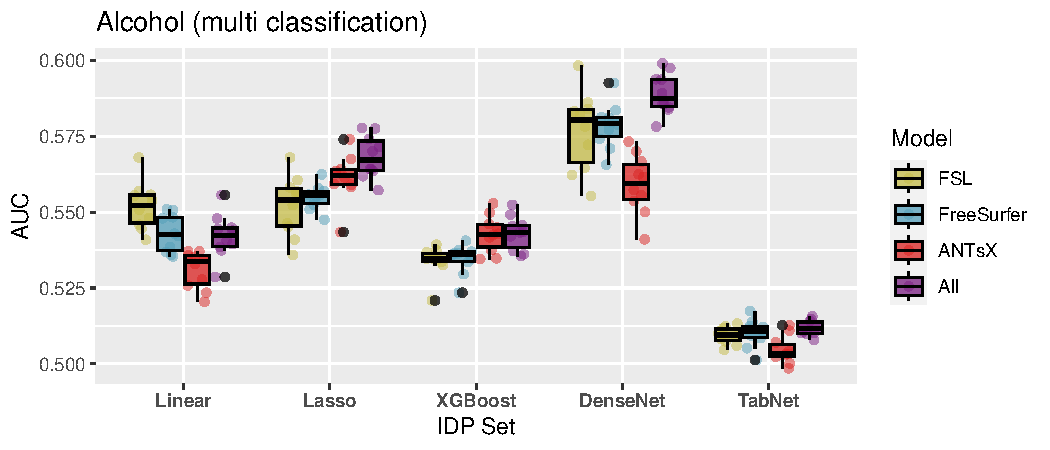
\includegraphics{/Users/ntustison/Documents/Academic/InProgress/ANTsXUKBB/Text/Figures/compare_predictions_Alcohol.pdf}
\caption{Alcohol}
\end{figure}

\hypertarget{feature-ranking-linear-11}{%
\subsection{Feature ranking: Linear}\label{feature-ranking-linear-11}}

\begin{table}

\caption{\label{tab:compare-predictions}Alcohol}
\centering
\begin{tabular}[t]{lll}
\toprule
Package & Pipeline & Feature\\
\midrule
FreeSurfer & ASEG & Volume of Thalamus-Proper (right hemisphere)\\
ANTsX & Atropos & DeepGrayMatter\\
FreeSurfer & ASEG & Volume of Pallidum (left hemisphere)\\
-- & -- & NA\\
FreeSurfer & ASEG & Volume of Cortex (left hemisphere)\\
\addlinespace
FSL & Other & Continuous    Volume of brain = grey+white matter\\
FreeSurfer & ASEG & Volume of Hippocampus (left hemisphere)\\
ANTsX & Cereb & CerebellarGrayMatter volume\\
FreeSurfer & ASEG & Volume of CC-Central (whole brain)\\
ANTsX & Region & Right cerebellum white matter\\
\addlinespace
FSL & Other & Continuous    Volume of ventricular cerebrospinal fluid (normalised for head size)\\
FreeSurfer & ASEG & Volume of VentralDC (right hemisphere)\\
FreeSurfer & ASEG & Volume of Thalamus-Proper (left hemisphere)\\
FSL & Other & Continuous    Volume of ventricular cerebrospinal fluid\\
ANTsX & Region & Left amygdala\\
\addlinespace
FreeSurfer & ASEG & Volume of BrainSegNotVentSurf (whole brain)\\
ANTsX & Cortical & Left lingual volume\\
FSL & Other & Continuous    Volume of brain = grey+white matter (normalised for head size)\\
FSL & Other & Continuous    Volume of brain stem + 4th ventricle\\
ANTsX & Region & Left cerebellum white matter\\
\addlinespace
FSL & Other & Continuous    Volume of white matter\\
FSL & Other & Continuous    Volume of white matter (normalised for head size)\\
ANTsX & Cortical & Left superior temporal volume\\
FreeSurfer & ASEG & Volume of choroid-plexus (left hemisphere)\\
ANTsX & Region & Left transverse temporal\\
\bottomrule
\end{tabular}
\end{table}

\begin{itemize}
\item
  FSL

  \begin{itemize}
  \item
    range: {[} 0.0000000001192476 , 0.06011407 {]}
  \item
    std: 0.007067126
  \item
    skewness: 5.058123
  \end{itemize}
\item
  FreeSurfer

  \begin{itemize}
  \item
    range: {[} 0 , 0.1692415 {]}
  \item
    std: 0.01298998
  \item
    skewness: 8.804126
  \end{itemize}
\item
  ANTsX

  \begin{itemize}
  \item
    range: {[} 0 , 0.09457359 {]}
  \item
    std: 0.007797607
  \item
    skewness: 7.256026
  \end{itemize}
\end{itemize}

\hypertarget{package-based-ranking-top-10-features-11}{%
\subsubsection{Package-based ranking (top 10
features)}\label{package-based-ranking-top-10-features-11}}

\begin{itemize}
\item
  FSL: rank = 233 , imp = 0.2657077
\item
  FreeSurfer: rank = 116 , imp = 0.5770373
\item
  ANTsX: rank = 177 , imp = 0.3491997
\end{itemize}

\hypertarget{package-based-ranking-top-25-features-11}{%
\subsubsection{Package-based ranking (top 25
features)}\label{package-based-ranking-top-25-features-11}}

\begin{itemize}
\item
  FSL: rank = 1447 , imp = 0.3594325
\item
  FreeSurfer: rank = 869 , imp = 0.7370469
\item
  ANTsX: rank = 840 , imp = 0.5216603
\end{itemize}

\hypertarget{package-based-ranking-top-50-features-11}{%
\subsubsection{Package-based ranking (top 50
features)}\label{package-based-ranking-top-50-features-11}}

\begin{itemize}
\item
  FSL: rank = 4873 , imp = 0.4520167
\item
  FreeSurfer: rank = 4545 , imp = 0.8297048
\item
  ANTsX: rank = 2926 , imp = 0.675435
\end{itemize}

\clearpage

\begin{center}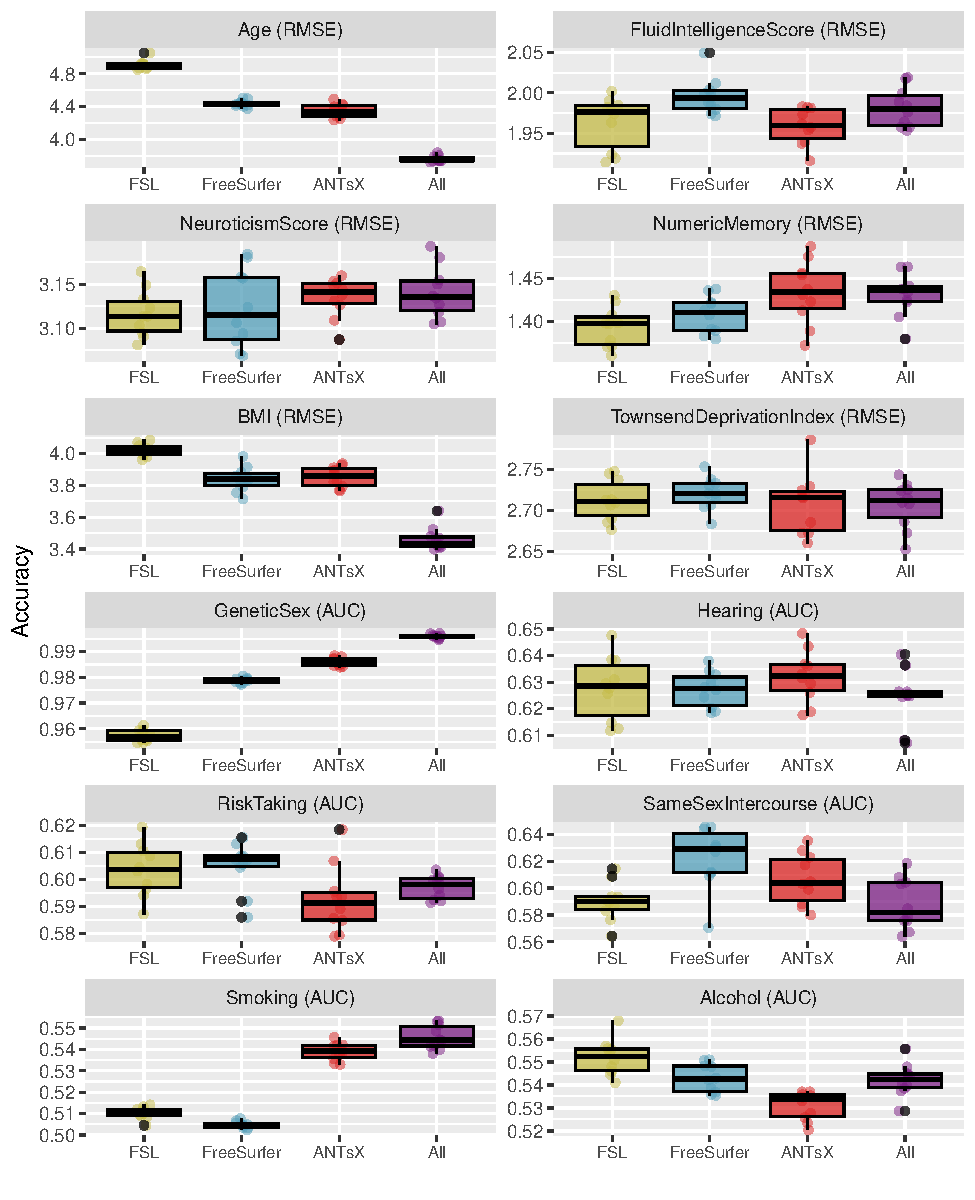
\includegraphics{../Text/Figures/compare_predictions_all} 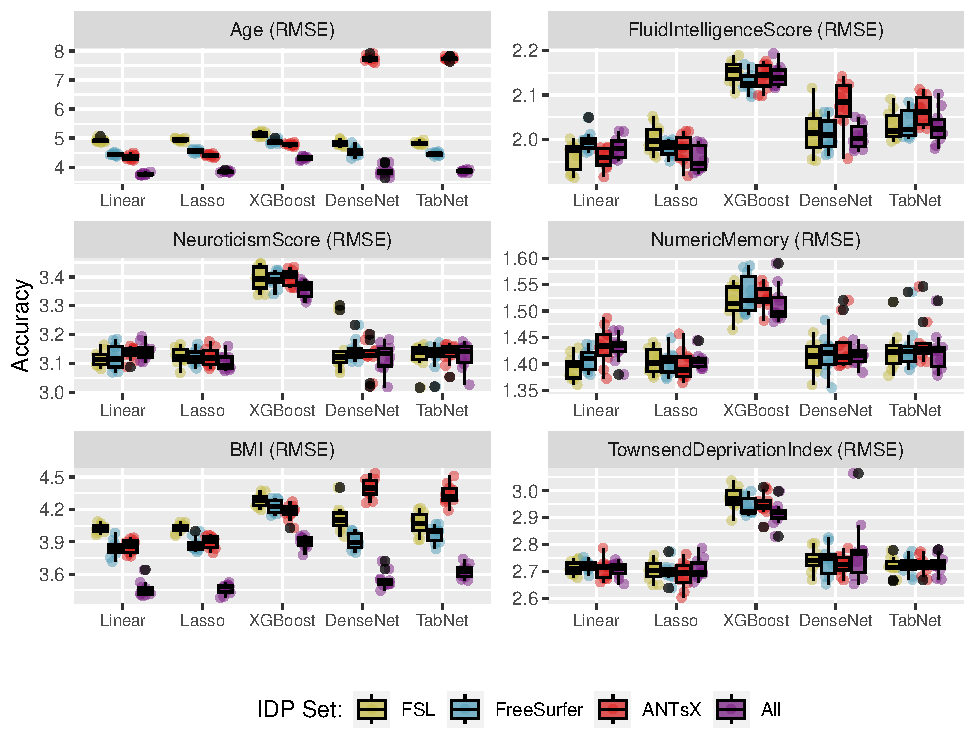
\includegraphics{../Text/Figures/compare_predictions_rmse} 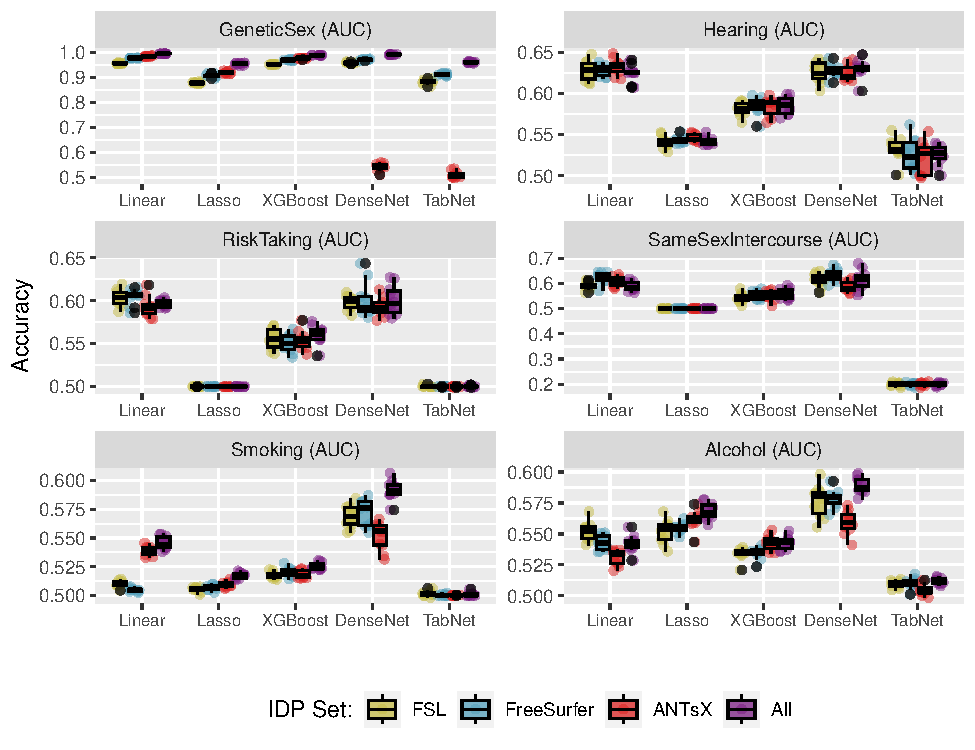
\includegraphics{../Text/Figures/compare_predictions_auc} \end{center}

\end{document}
